\documentclass[11pt]{article}
\usepackage[utf8]{inputenc}

\usepackage[export]{adjustbox}
\usepackage{colortbl}
\usepackage{fancyvrb}
\usepackage{float}
\usepackage[margin=1in]{geometry}
\usepackage{graphicx}
\usepackage{hyperref}
\usepackage{indentfirst}
\usepackage{listings}
\usepackage{spverbatim}
\usepackage{subcaption}
\usepackage{tikz}
\usepackage{tocloft}
\usepackage{xcolor}


\title{DSSG BCCDC Final Report}

% Rename table of contents
\renewcommand*\contentsname{Table of Contents}
% Table of content dots
\renewcommand{\cftsecleader}{\cftdotfill{\cftdotsep}}
% Clickable table of contents
\hypersetup{allcolors=black}

% Line spacing
\renewcommand{\baselinestretch}{1.25}

% Paper width image definition
\newcommand{\adjustimg}{% Horizontal adjustment of image
  \checkoddpage%
  \ifoddpage\hspace*{\dimexpr\evensidemargin-\oddsidemargin}\else\hspace*{-\dimexpr\evensidemargin-\oddsidemargin}\fi%
}
\newcommand{\centerimg}[2][width=\textwidth]{% Center an image
  \makebox[\textwidth]{\adjustimg\includegraphics[#1]{#2}}%
}


\newcommand{\MyGraphicLogo}{% For imported graphic logo
\begin{tikzpicture}[remember picture,overlay,yshift=-2cm, xshift=2cm]
  \node at (0,0) {\includegraphics[width=2cm,height=2cm]{foo}};
 \end{tikzpicture}
}


% Table colours
\definecolor{Gray}{gray}{0.85}
\definecolor{LightGray}{gray}{0.98}
\newcolumntype{g}{>{\columncolor{Gray}}c}


\begin{document}

% Title page
\begin{titlepage}
    \centering
    \rule{\linewidth}{0.5 mm} \\[0.6 cm]
    \textsc{\Large Classifying Laboratory Test Results Using Machine Learning}\\[0.4cm]
    \rule{\linewidth}{0.5 mm} \\[0.5 cm]
    
        \begin{minipage}{\textwidth}
        \centering
        Sizhe Chen \hspace*{1cm} Kenny Chiu \hspace*{1cm} William Lu \hspace*{1cm} Nilgoon Zarei
    \end{minipage}
    
    \vspace*{1cm}
    \mbox{}\par\noindent\centerimg[width=\textwidth,height=170pt]{title_pic}
    
    \vspace*{1cm}
    
    \textsc{\large The University of British Columbia}\\
    \vspace{0.2cm}
    \textsc{\large Data Science for Social Good Fellowship 2018}\\[1cm]
   
    \textsc{in partnership with}\\
    \vspace{0.2cm}
    \textsc{\large The BC Centre for Disease Control}\\
    
    \vspace{4.2cm}
    
    \begin{figure}[h]
        \begin{minipage}{0.36\textwidth}
        \hspace*{5.5cm}\includegraphics[height=1.4cm,right]{UBC_logo.png} 
       
        \end{minipage}
        \begin{minipage}{0.22\textwidth}
        \hspace*{5.5cm}\includegraphics[height=1.4cm,right]{CDC_logo.jpg} 
       
        \end{minipage}
        \begin{minipage}{0.09\textwidth}
        \vspace{-0.1cm}\hspace*{5.5cm}\includegraphics[height=1.6cm,right]{Microsoft_Logo.png}
       
        \end{minipage}
    \end{figure}

\end{titlepage}


\newpage

% Table of contents
\tableofcontents

\newpage


\section{Introduction} \label{introduction}

This report was the result of the collaboration between the University of British Columbia's (UBC) Data Science for Social Good (DSSG) 2018 program and the BC Centre for Disease Control (BCCDC). In this section, we introduce the two parties involved and summarize the project context and goals. In Section \ref{literature review}, we provide a brief overview of related work in literature. We share the main results of our analysis in Sections \ref{results and analysis} and \ref{pipeline architecture} before concluding this report with some discussion and comments in Section \ref{discussion}.


\subsection{Data Science for Social Good} \label{data science for social good}

The DSSG program is a 14-week fellowship that is offered by the UBC Data Science Institute (DSI) and sponsored by Microsoft. The program is designed to provide UBC undergraduate and graduate students of diverse backgrounds the experience of working on a data science project that pertains to the concept of ``social good". While the concept in itself may be broad and abstract, these projects are generally brought forth by nonprofit organizations or organizations in the public sector and make use of data to benefit society and improve people's well-being in some aspect. Through the program, the students have the opportunity to learn and apply data science, and the organizations have the opportunity to make progress on these projects with minimal resources.


\subsection{Background} \label{background}

Operated by one of BC's health authorities, the BCCDC provides several health-care services including:

\begin{itemize}

\item managing various health clinics and laboratories throughout BC

\item providing programs that contribute to public health

\item analyzing and monitoring disease trends at the population level

\end{itemize}

\noindent Through their services, the BCCDC has collected over twenty years of patient and laboratory test result data. As part of their work in analyzing disease trends, it is now in their interest to review the historical laboratory tests and extract various pieces of information such as the purpose of the test, the microorganism that is being tested for, and the outcome of the test. However, this process of labeling each test result is currently being performed manually, and is expensive to carry out for the following reasons:

\begin{enumerate}

\item[1.] The test result description text can be difficult to interpret

\end{enumerate}

The laboratory test results are stored as semi-structured text in their data warehouse. The semi-structure form is the consequence of the laboratory technician having the option of either inputting a code that auto-generates the text, inputting completely free-form text, or inputting a combination of the two where free-form text is appended to auto-generated text. As a result, there is no consistent structure in the test results that can allow for simple rule-based processing.
\\

In addition, the actual content of the text further complicates the issue more. Unlike standard natural language documents, the test results are often recorded in point-form and are mostly composed of laboratory-specific terminology including microorganism names, laboratory procedure names, and abbreviations. It is also not uncommon that the entirety of the text is a single number, or that the free-form text contains typographical errors. The free-form text may also include information such as names and phone numbers that may require special attention during processing. Figure \ref{test results figure} shows examples of what a test result description may contain.

\begin{figure}
    \centering
    \includegraphics[width=12cm]{rfd_ex.png}
    \caption{Examples of laboratory test results.}
    \label{test results figure}
\end{figure}


\begin{enumerate}

\item[2.] There is a high-volume of test results that still need to be interpreted and labeled

\end{enumerate}

BCCDC's data warehouse contains over 330 million test results. As of the time of this report, they have labeled only a subset of the data that is relevant to some of their data marts. Manually going through the large number of remaining unlabeled test results along with the new test results that are added each day would require additional resources that are simply not available.


\subsection{Project Goals and Scope} \label{project goals and scope}

The process of manually labeling the test results in BCCDC's data warehouse is expensive to carry out. Thus, the goal of this project is to achieve the following objectives:

\begin{enumerate}

\item[G1.] To identify the appropriate machine learning or natural language processing (NLP) solutions for automating the labeling process

\item[G2.] To provide an example code solution implementing G1 that can be integrated into the extract, transform, and load process of the data warehouse

\item[G3.] To recommend changes in how the data is stored to improve the efficiency of the labeling process

\end{enumerate}

\noindent This report focuses on the work that we associate with G1. Specifically, we evaluate algorithms for labeling the outputs of interest shown in Table \ref{outputs of interest}. Our code solution for G2 is detailed in a separate technical documentation produced along with this report. Section \ref{recommendations for the bccdc} provides a summary of our recommendations for G3.
\\

\begin{table}[ht]
\begin{center}
\begin{tabular}{|c|l|c|}
    \hline
    \rowcolor{Gray}
    \textbf{Output} & \textbf{Description} & \textbf{Classes} \\
    \hline
    \verb|test_performed| & whether the test was performed & \begin{tabular}{@{}c@{}}\textit{Yes} \\ \textit{No}\end{tabular} \\
    \hline
    \rowcolor{LightGray}
    \verb|test_outcome| & whether the microorganism being tested for was found & \begin{tabular}{@{}c@{}}\textit{Positive} \\ \textit{Negative} \\ \textit{Indeterminate} \\ \textit{Missing}\end{tabular} \\
    \hline
    \verb|level_1| & the genus name of the microorganism being tested & 30 classes and counting \\
    \hline
    \rowcolor{LightGray}
    \verb|level_2| & the species name of the microorganism being tested & 200 classes and counting \\
    \hline
\end{tabular}
\caption{The outputs to label for each test result.}
\label{outputs of interest}
\end{center}
\end{table}


\section{Literature Review} \label{literature review}

%TODO: https://www.ncbi.nlm.nih.gov/pmc/articles/PMC3779392/; http://www.cs.cmu.edu/~hyejuj/papers/2006.10-Jang.pdf; https://www.sciencedirect.com/science/article/pii/S1386505614001105
% everything written here is based off of skimming through the article, someone should review and double check
% also fix reference format and style

We provide a brief overview of similar work in literature in this section. In 2014, Kang and Kayaalp explored the problem of extracting laboratory test information from biomedical text and compared the performance of an original symbolic information extraction (SIE) system to various machine learning-based NLP systems [2]. Their results showed that well-tailored symbolic approaches may outperform machine learning-based approaches. The main difference between our problem and theirs is that the document corpus they extract from are decision summaries from the U.S. Food and Drug Administration. These summaries are written in natural language unlike our test result descriptions which are found mostly in point-form. We expect that this difference will be significant enough that a symbolic approach to our problem will require more complex logic before it can achieve similar results to theirs.
\\

Jang et al. used hidden Markov models to text mine doctor notes in 2006 [1]. The document corpus that they worked with were more challenging as the notes were written in a mixture of English and Korean. Their models achieved around 60\%-70\% accuracy and aimed to be robust to unknown phrases not seen in the training corpus. One notable tool that they also used is \textit{MetaMap}, which can be used to annotate input text with medical tags and semantics. MetaMap is also commonly used in other health domains such as for text mining of cancer-related information [3].


\section{Dataset} \label{dataset}

The dataset that we work with was provided in the form of multiple tables in a Microsoft SQL Server 2016 database. The dataset is a subset of the data available in BCCDC's data warehouse and consists of approximately 950,000 test results. The test results were selected in a way such that the majority contain no personally identifiable information. Not all test results in the dataset are labeled. Figure \ref{proportion of labeled data figure} in Appendix \ref{proportion of labeled data} shows the proportion of labeled data for each output. We note that the proportions vary significantly ranging from 100\% in the case of \verb|test_performed| to around 11\% for the microorganism name outputs.
\\

Figure \ref{class breakdown of labeled data figure} in Appendix \ref{class breakdown of labeled data} shows the class breakdown of labeled data for each output. We observe that \verb|test_performed| has severe class imbalance, with 94\% of the labeled rows being \textit{Yes}. \verb|test_outcome| also has severe class imbalance between 69\% of the labeled rows being \textit{Missing} and 1\% \textit{Indeterminate}. We also note that there are some \verb|level_1| classes with very few rows in the dataset. The smallest class has only 50 rows.
\\

We will refer to the data fields shown in Table \ref{data fields} frequently throughout our analysis in Section \ref{results and analysis}.
\\

\begin{table}[ht]
\begin{center}
\begin{tabular}{|c|p{9.5cm}|}
    \hline
    \rowcolor{Gray}
    \textbf{Data Field} & \textbf{Description} \\
    \hline
    \verb|result_full_description| (RFD) & the full test result text. A RFD may consist of multiple observations \\
    \hline
    \rowcolor{LightGray}
    \verb|test_type| & describes the type of test, e.g. \verb|Culture| for culture tests \\
    \hline
    \verb|test_code| & the code for the name of the test, e.g. \verb|CULT| for some culture tests \\
    \hline
    \rowcolor{LightGray}
    \verb|obs_seq_nbr| & the sequence number in which the observation appears in the RFD \\
    \hline
\end{tabular}
\caption{The relevant data fields we use in our analysis.}
\label{data fields}
\end{center}
\end{table}


\section{Results and Analysis} \label{results and analysis}

We highlight our key analysis and results in this section. Our analysis was primarily carried out using Python 3.6 with the MetaMap components done in Java 10.


\subsection{Preliminary Analysis} \label{preliminary analysis}

Before we explore possible solutions to our main problem, we first run simple queries to get a better sense of what the data consists of. In particular, we attempt to identify common patterns in the RFD fields of the test results. A word cloud of the most frequently occurring words in the RFD's is shown in Figure \ref{most frequent words figure}. Stop-words (common English words that do not provide much insight such as ``the" or ``and") were removed prior to the generation of the word cloud. We observe that the remaining most frequent words are generally biological, medical, or laboratory terminology such as ``specimen", ``assay", and ``reactive". We also note the presence of abbreviations such as ``hiv" and ``hbv", and lab techniques such as ``pcr".

\begin{figure}
    \centering
    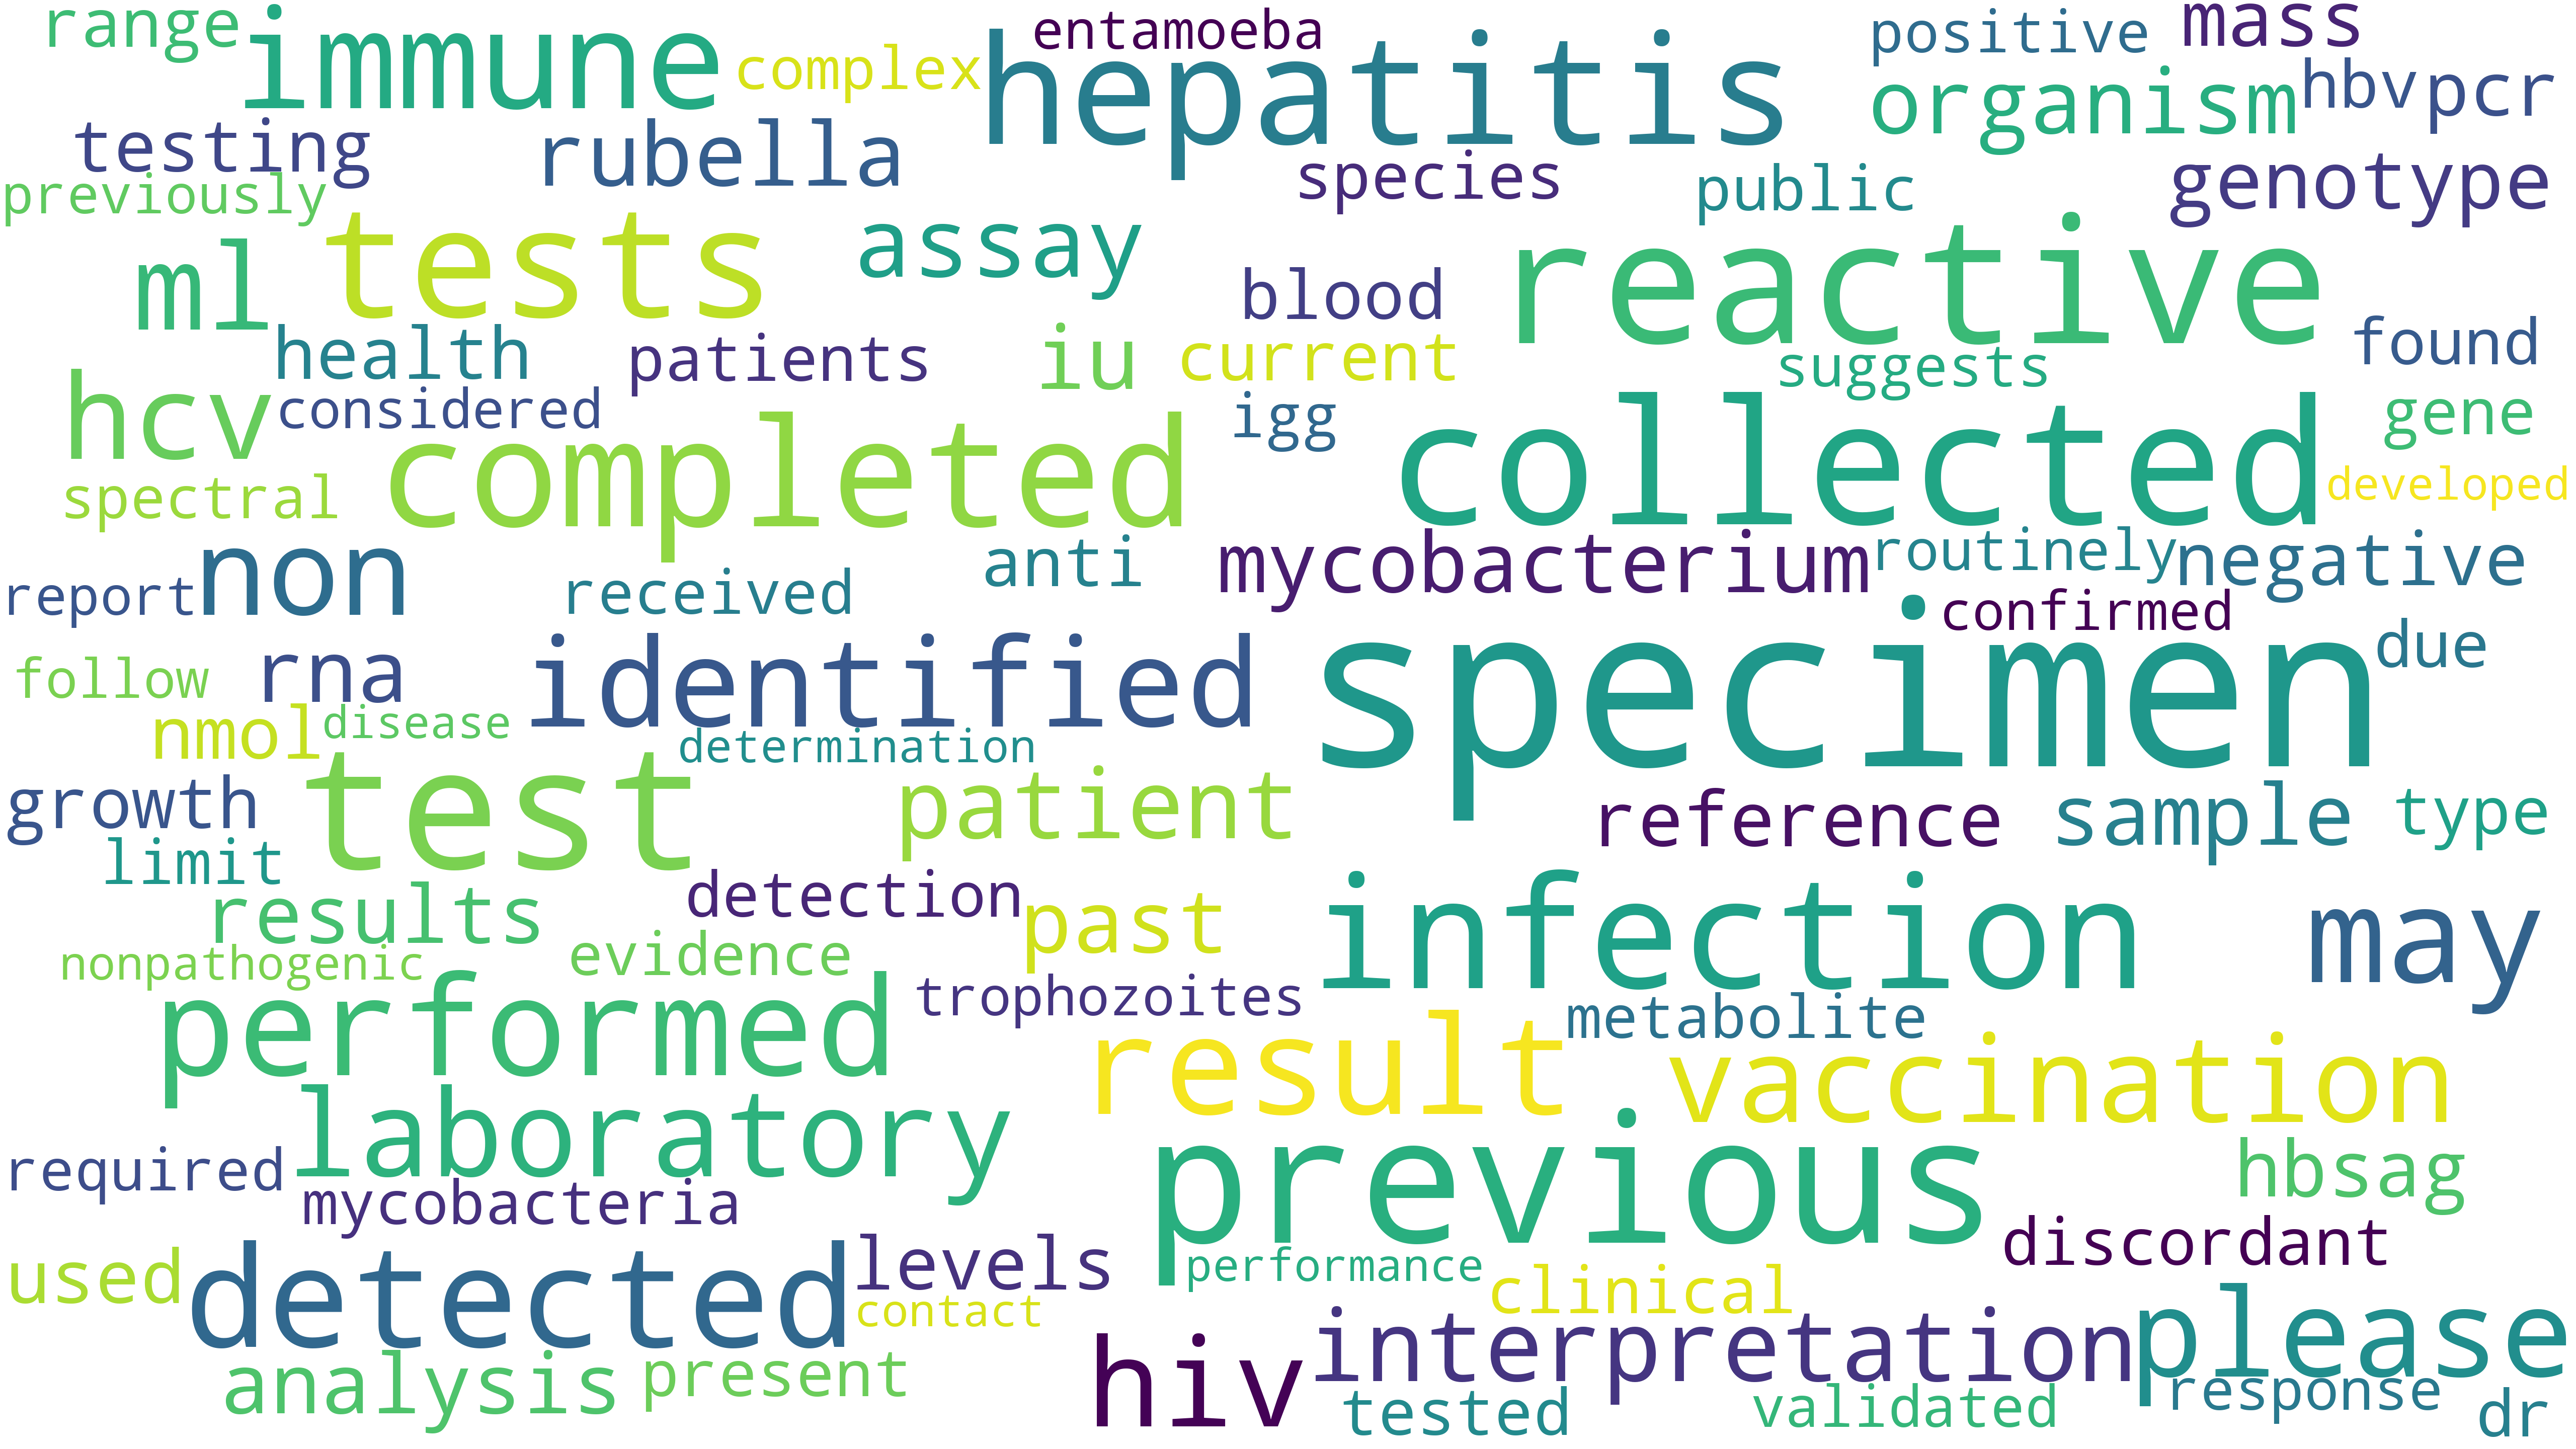
\includegraphics[width=\textwidth]{dataset.png} \\
    \caption{A word cloud of the most frequently occurring words in the RFD's (stop-words removed).}
    \label{most frequent words figure}
\end{figure}


\subsection{Baseline Machine Learning Classifiers} \label{baseline machine learning classifiers}

We determined that a machine learning approach would not be appropriate for \verb|level_2| due to the number of classes and some classes having only one example in our dataset. We revisit \verb|level_2| in Section \ref{symbolic approach to microorganism name}.
\\

We start by experimenting with standard machine learning classifiers using only the RFD field for the \verb|test_performed|, \verb|test_outcome| and \verb|level_1| outputs. We describe our data preprocessing procedure in Section \ref{data preprocessing} and summarize the results in Section \ref{classifier results}.


\subsubsection{Data Preprocessing} \label{data preprocessing}

Due to the presence of free-form text in the RFD's, there are many issues with the content that would be problematic if we were to train machine learning classifiers using the RFD's as-is. For example, many RFD's consist of a single number or contain meaningless symbols. We start by cleaning and transforming the data into a usable form.
\\

We start by removing all the empty RFD's and RFD's consisting of only a single number from our dataset. For the remaining RFD's, we remove all irrelevant symbol characters (e.g. `\verb|_|') from the text. We then replace all standalone numbers (e.g. ``16") by a special token to prevent our classifiers from overfitting to specific number values. Lower-casing the existing test result labels is also necessary as there are inconsistencies such as `\verb|Yes|' and `\verb|yes|'. Another potential issue in the data is the presence of specific dates in different formats. We choose to ignore the dates due to the lack of time and usable tools that could identify all the differing forms of a date. In future work, it may be reasonable to replace all dates by a special date token similar to what we did with numbers.
\\

After cleaning the data, we transform the RFD's into numeric vectors using the \textit{bag-of-words} representation and drop the low frequency tokens (less than 10 occurrences in our analysis). We experimented with other representations such as TF-IDF and positioning-based forms, but found no significant differences in the results between using those and bag-of-words. For \verb|test_performed|, we find that using unigrams to trigrams resulted in the best performance while there is little to no difference compared to just using unigrams for the other outputs.


\subsubsection{Classifier Results} \label{classifier results}

The standard machine learning classifiers we experiment with include \textit{na\"ive Bayes} (NB), L2-regularized \textit{logistic regression} (LR), 100-tree \textit{random forest} (RF), and linear-kernel \textit{support vector machine} (SVM). To evaluate the classifiers, we perform 5-fold cross validation and average the test accuracy across the five folds. The classifiers achieve high test accuracies in the case of \verb|test_performed| as seen in Figure \ref{test performed figure}. The trigram ``test not performed" is seen to be the strongest predictor across all our models. Close inspection of the resulting confusion matrices however show symptoms of bias towards the majority class. We address this issue in Section \ref{class imbalance}.
\\

\begin{figure}[H]
    \centering
    \includegraphics[width=8cm]{tp_graph.png} \\
    \SaveVerb{test performed}|test_performed|
    \caption{Baseline classifier performances for \protect\UseVerb{test performed}.}
    \label{test performed figure}
\end{figure}

In the case of \verb|test_outcome|, the standard machine learning classifiers achieve similar results. The previously mentioned class imbalance issue does not appear to significantly impact results for \verb|test outcome|. Figure \ref{test outcome figure} shows the classifiers achieve around 95\% test accuracy for NB and around 99\% for the others.
\\

\begin{figure}[H]
    \centering
    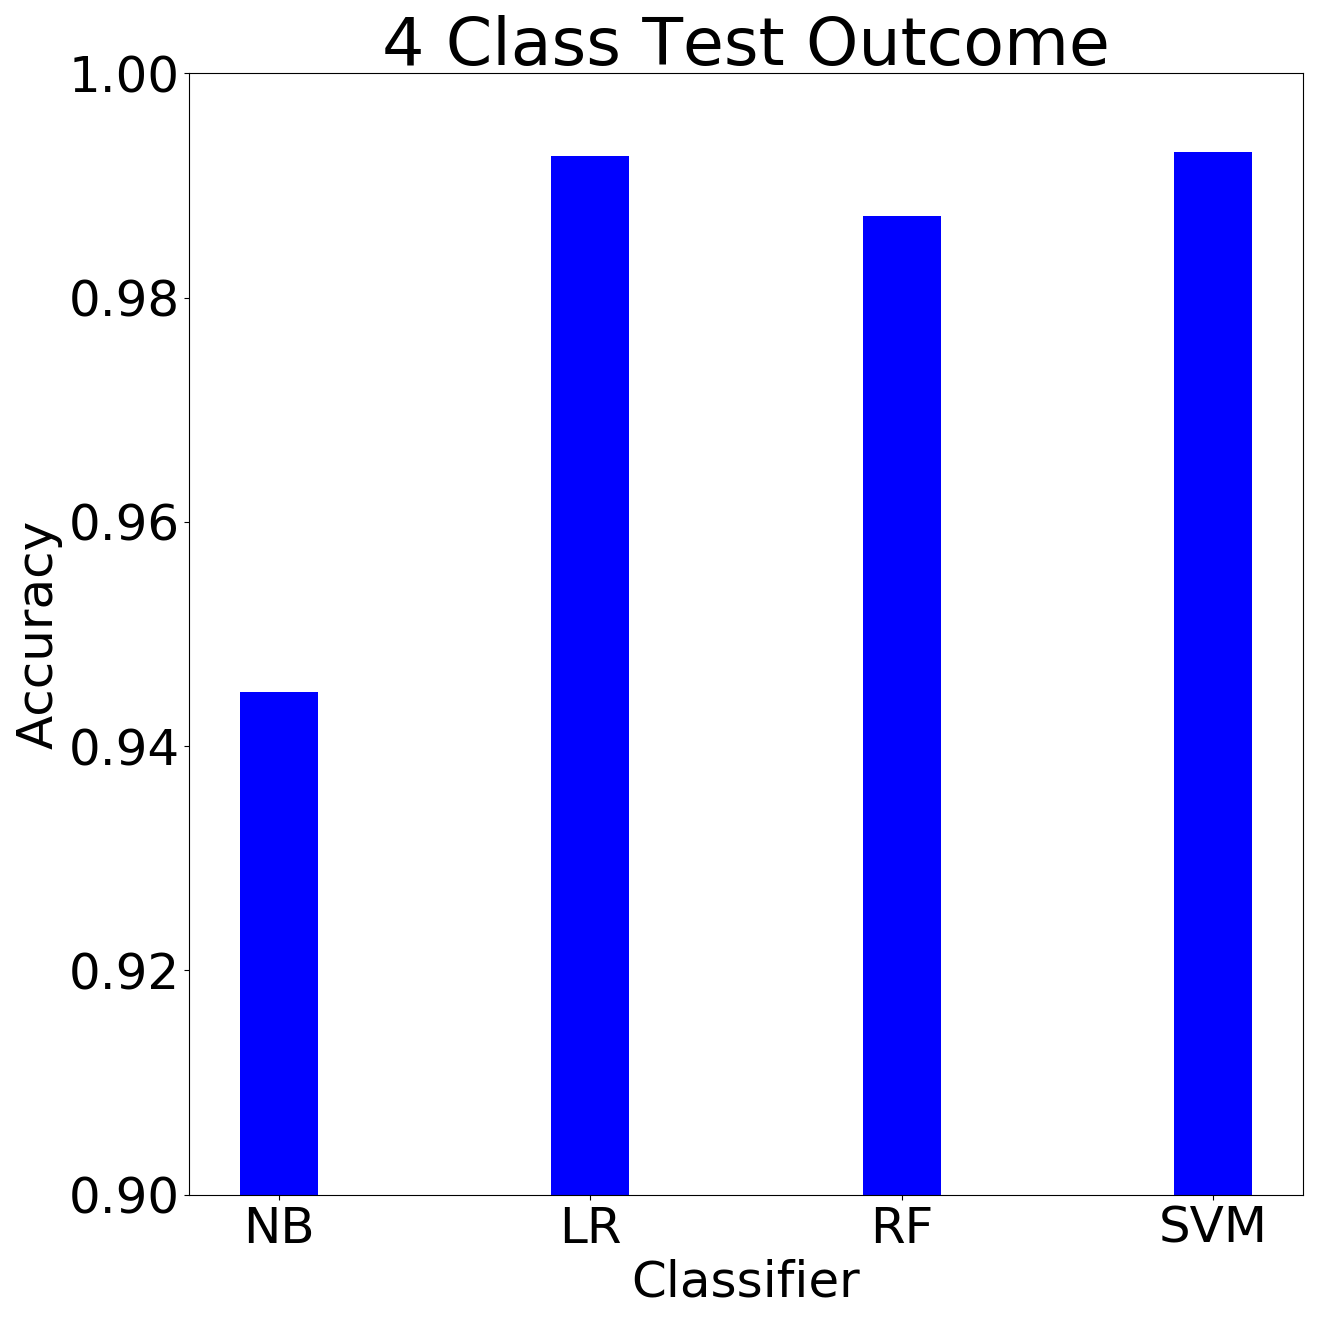
\includegraphics[width=8cm]{to_4c_graph.png} \\
    \SaveVerb{test outcome}|test_outcome|
    \caption{Baseline classifier performances for \protect\UseVerb{test outcome}.}
    \label{test outcome figure}
\end{figure}

The \verb|test_outcome| classifiers retain their high accuracy scores even when feature selection is done to reduce the size of the feature space. We opted for \verb|scikit|'s chi-square feature selection algorithm for ease of use and convenience. From Figure \ref{test outcome chi2 figure}, we see that only around 150 features are required for the performance of the LR, RF, and SVM classifiers to asymptote. We see a similar trend in the case of \verb|test_performed|.
\\

\begin{figure}[H]
    \centering
    \includegraphics[width=12cm]{to4c_chi2_trend_newest.png} \\
    \SaveVerb{test outcome}|test_outcome|
    \caption{Test accuracy versus number of features retained for \protect\UseVerb{test outcome}.}
    \label{test outcome chi2 figure}
\end{figure}

From Figure \ref{test outcome size figure}, we observe that the \verb|test_outcome| classifiers also retain their accuracy when the training and test set sizes are reduced. This indicates that our text data may contain more structure than we initially expected. Intuitively, this structure may be due to certain snippets of the text that were auto-generated from standardized lab codes.
\\

\begin{figure}[H]
    \centering
    \includegraphics[width=12cm]{to4c_trend_newest.png} \\
    \SaveVerb{test outcome}|test_outcome|
    \caption{Test accuracy versus size of training set for \protect\UseVerb{test outcome}.}
    \label{test outcome size figure}
\end{figure}

Error analysis shows that many of the misclassified test results contain contradictory RFD's, where observations at the start are discordant with observations at the end. For example, the RFD

\begin{quotation}
\noindent \textit{Bordetella pertussis DNA detected by PCR. $\vert$ CORRECTED ON 14/Oct AT 1554: PREVIOUSLY REPORTED AS No Bordetella pertussis DNA detected by PCR. $\vert$ Culture results to follow.}
\end{quotation}

\noindent is interpreted as ``\textit{Bordetella pertussis} DNA was actually detected despite being previously reported as not detected". Our classifiers struggle more with cases like this one where they predict \textit{Negative} for \verb|test_outcome| when the true label is \textit{Positive}. We also note though that our classifiers do correctly classify a significant number of these contradictory test results, and correctly classify the majority of the non-contradictory test results.
\\

The standard machine learning classifiers also achieve high test accuracies for \verb|level_1|. The recall and precision scores vary greatly between classes, where the classifiers appear to predict better on the classes having more data and more structured RFD's. The important features as reported by RF consist mostly of organism-specific terms such as ``salmonella", ``streptococcus", and ``hiv". This provides some support that our classifiers are learning reasonable patterns for predicting \verb|level_1|. However, we also reconsider the use of machine learning for labeling \verb|level_1|. We save this discussion until after we revisit \verb|level_1| in Sections \ref{symbolic approach to microorganism name} and \ref{machine learning versus symbolic}.


\subsection{Class Imbalance} \label{class imbalance}

The \verb|test_performed| classifiers achieved high test accuracies (i.e. well above 95\%). Upon closer investigation however, the resulting confusion matrices show signs that our classifiers are heavily biased toward the majority class \textit{Yes}. Table \ref{class imbalance table} shows the confusion matrix for one of the folds. Specifically, note that the recall score for rows with true class \textit{No} is 79\%, which is noticeably lower than the other scores.
\\

\begin{table}[ht]
\begin{center}
\begin{tabular}{|g|c|c|c|}
    \hline
    \rowcolor{Gray}
    & \textbf{Predicted \textit{Yes}} & \textbf{Predicted \textit{No}} & \textbf{Recall} \\
    \hline
    \textbf{True \textit{Yes}} & 67,696 & 411 & 99\%  \\
    \hline
    \textbf{True \textit{No}} & 947 & 3,475 & 79\%\\
    \hline
    \textbf{Precision} & 99\% & 89\% & \\
    \hline
\end{tabular}
\SaveVerb{testperf}|test_performed|
\caption{The \protect\UseVerb{testperf} confusion matrix for one of the folds.}
\label{class imbalance table}
\end{center}
\end{table}

%                      Pred. yes        Pred. no           Recall
%True yes                 67696             411              99%
%True no                   947              3475             79%
%Precision                99%               89%

We consider three possible solutions for the class imbalance problem observed in the baseline result.

\begin{enumerate}

\item
\textit{Downsampling}, where rows with true class \textit{Yes} are randomly removed from the training set until the training set is balanced. The disadvantage of this approach is that due too how imbalanced the classes are, much of the data is left unused. This can also lead to an overfitting problem where the classifiers only learn patterns from the few remaining data that is left to train on.

\item
\textit{Upsampling}, where rows with true class \textit{No} are randomly duplicated in the training set until the training set is balanced. The disadvantage of this approach is the impact on training time. By duplicating rows until the training set is balanced, we are almost doubling the size of the training set.

\item
\textit{Class weighting}, where we introduce heavy penalties (weights) when the classifier misclassifies the minority class during training. One point to consider with this approach is the choice of weights. Because the weights may be arbitrarily chosen, it is arguable that this approach introduces a bias that may or may not be non-trivial.

\end{enumerate}

We find that the approaches above reduce the number of false positives (rows with true class \textit{Yes} that are predicted as \textit{No}), but do so at the expense of introducing many more false negatives (rows with true class \textit{No} that are predicted as \textit{Yes}). Table \ref{class weighting table} shows the confusion matrix for one of the folds when the classes are weighted. In particular, the recall score for rows with true class \textit{No} improves, but the precision score for rows with predicted class \textit{No} decreases.
\\

\begin{table}[ht]
\begin{center}
\begin{tabular}{|g|c|c|c|}
    \hline
    \rowcolor{Gray}
    & \textbf{Predicted \textit{Yes}} & \textbf{Predicted \textit{No}} & \textbf{Recall} \\
    \hline
    \textbf{True \textit{Yes}} & 66,355 & 1,800 & 97\%  \\
    \hline
    \textbf{True \textit{No}} & 429 & 3,945 & 90\%\\
    \hline
    \textbf{Precision} & 99\% & 69\% & \\
    \hline
\end{tabular}
\SaveVerb{testperf}|test_performed|
\caption{The \protect\UseVerb{testperf} confusion matrix for one fold when class weighting is used.}
\label{class weighting table}
\end{center}
\end{table}

%                      Pred. yes        Pred. no           Recall
%True yes                 66355             1800              97%
%True no                   429              3945             90%
%Precision                99%               69%

We consulted a domain expert and determined that false positives are more acceptable than false negatives. Hence we retain the original \verb|test_performed| classifiers without the additional solutions for addressing class imbalance in our pipeline code.


\subsection{MetaMap} \label{metamap}

MetaMap is a tool that can identify and annotate input text based on concepts in the Unified Medical Language System (UMLS) medical vocabulary. In particular, MetaMap can identify words as concepts within specific \textit{Semantic Types} such as \textit{Finding} or \textit{Bacterium}. Figure \ref{metamap example figure} shows an example of MetaMap's annotation. Further details regarding MetaMap's output can be found in our separate \textbf{MetaMapBuild Source Code Documentation} produced along with this report.
\\

\begin{figure}[H]
    \centering
    \includegraphics[scale=0.8]{MetaMap_tag_sample.png}

    \caption{Example of concepts (yellow) and corresponding \textit{Semantic Types} identified by MetaMap.}
    \label{metamap example figure}
\end{figure}

\iffalse
For example, when MetaMap is run on the following string: \begin{spverbatim}
"Rhinovirus or Enterovirus detected by multiplex NAT. Adenovirus detected by multiplex NAT. Multiplex NAT is capable of detecting Influenza A and B, Respiratory Syncytial Virus, Parainfluenza 1, 2, 3, and 4, Rhinovirus, Enterovirus, Adenovirus, Coronaviruses HKU1, NL63, OC43, 229E, hMetapneumovirus, Bocavirus, C. pneumoniae, L. pneumophila, and M. pneumoniae. MULTIPLE INFECTION DETECTED"
\end{spverbatim}
\medskip
The organisms ``Coryza Viruses", ``Respiratory syncytial virus", ``Bocavirus", ``Adenoviruses", ``Mycoplasma pneumoniae", ``Legionella pneumophila", ``Enterovirus", ``Genus: Coronavirus", and ``Rhinovirus" are detected by MetaMap.
\fi

We experiment with MetaMap in an attempt to improve the generalizability of our classifiers. As part of the preprocessing procedure, we send all the RFD's to MetaMap and store the annotations for each RFD. We then apply the unigram bag-of-words transformation on only the annotations, which results in a feature set of approximately 100 unique semantic types. The classifiers trained on this feature set achieve approximately 95\% test accuracy, which is slightly worse than what our baseline classifiers achieved. However, the classifiers also do not appear to generalize as well as expected to simple example sentences that we create. Further analysis shows that perhaps some of the MetaMap annotations are too general and that using only the annotations results in significant loss of meaning. For example, the words ``positive" and ``negative" are both annotated as \textit{Finding}. The semantics of these words would be important particularly in the case of \verb|test_outcome|, and so the generalization from MetaMap does more harm than good in situations like this.


\subsection{Symbolic Approach to Microorganism Name} \label{symbolic approach to microorganism name}

Though using the MetaMap annotations as features did not improve the performance of our classifiers, we recognize that there may be value in MetaMap for other approaches. In particular, we consider a non-machine learning approach for labeling the \verb|level_1| and \verb|level_2| outputs.
\\

In what we call the symbolic approach, we again use MetaMap to annotate the RFD's. For each RFD, we then collect all the terms in which MetaMap identified as \textit{Bacterium} or \textit{Virus} into a \textit{candidates} list. Our output label would then be one of the names in the candidates. The advantage of using MetaMap here is that not only can it recognize microorganism names as an entity, it can also recognize abbreviations of the names (e.g. \textit{E. coli}) and map them to their full \textit{preferred} name (e.g. \textit{Escherichia coli}).
\\


The crucial step in this approach is how the final label is chosen from the candidates. In our algorithm, we use a pre-constructed dictionary based on the existing \verb|level_1| and \verb|level_2| labels. If a name in the candidates exists in the dictionary, we prioritize that name as the output. Otherwise we arbitrarily pick a name from the candidates. While this approach is somewhat na\"ive, we obtain 90\% accuracy on \verb|level_1| and 50\% accuracy on \verb|level_2|.


\subsubsection{Machine Learning Versus Symbolic} \label{machine learning versus symbolic}

We have tried both a machine learning approach and a symbolic approach for \verb|level_1| and \verb|level_2|. We briefly discuss the advantages and disadvantages of both approaches in this section.
\\

The machine learning approach has shown better performance on the microorganism name outputs overall. The approach also requires minimal manual configuration and is simple to implement. However, the key downside is that the trained classifier cannot label previously unseen microorganism names. How the classifier is labeling the microorganism name can also be difficult to interpret and adjust if desirable to do so.
\\

Our symbolic approach does not do as well compared to the machine learning approach. The algorithm also fails when a microorganism is detected but its name does not appear in the test RFD. On the other hand, the approach does allow the labeling of new microorganism names unlike the machine learning approach. The approach is also transparent in terms of how it is labeling the outputs, and can easily be modified to fit more complex algorithms to improve results.
\\

In summary, the machine learning approach performs better compared to our current symbolic algorithm, but the symbolic approach shows more promise as it can grow and be adjusted as needed. Specifically, the construction of the dictionary and how the algorithm chooses the label from the candidates are the key steps that have much potential for improvement.


\subsection{Unlabeled Data Evaluation} \label{unlabeled data evaluation}

To further evaluate our algorithms, we predict on new data and manually review the results with the BCCDC. The three sample datasets we use for this purpose include:

\begin{enumerate}

\item[D1.] An external set of 29 test results that the BCCDC had microorganism name previously labeled as \textit{Not in Hierarchy} that were re-labeled at a later date. It is expected that this set is most similar to the test results we have in our training dataset.

\item[D2.] A random sample of 100 unlabeled \verb|test_code| = \verb|CULT| test results in our dataset. It is expected that this set is somewhat similar to the labeled test results in our dataset which we are training on.

\item[D3.] A completely random sample of 100 unlabeled test results in our dataset. It is expected that there may be test results in this set that are very different from the ones we are training one.

\end{enumerate}

Based on our evaluation, the results can be summarized as follows.

\begin{enumerate}

\item[1.]
Our classifiers generally performed well on D1 except on \verb|test_outcome| where \textit{Missing} was the dominating (incorrect) label.

\item[2.]
Our classifiers did not perform well on D2 and D3. The \textit{Missing} \verb|test_outcome| issue is still present, and \textit{Not Found} is the dominating label for the microorganism name outputs.

\end{enumerate}

One hypothesis that we make is that our classifiers were overfitting to specific groups of test results, such as those involving \textit{Hepatitis C Virus}, because those groups are over-represented in our training dataset. Test results within these groups have very similar RFD's and labels, and so it is very likely that our classifiers try to correctly predict on these test results as much as possible. This might result in poor generalization to other test results that are lesser represented in our training set.


\subsection{Split by Test Type} \label{split by test type}

Our results from predicting on the new datasets showed that our classifiers seemed to be overfitting to certain subsets of test results that are over-represented in our dataset. To test our hypothesis that our dataset consists of test results from different ``true" distributions, we experiment by splitting our dataset into subsets where each subset contains test results of a certain \verb|test_type|.
\\

In particular, we consider the subset of \verb|Antibody| test results and the subset of \verb|NAT-PCR| test results. We train our classifier on the \verb|Antibody| subset and use it to make predictions on the \verb|NAT-PCR| subset. Our results show that the classifier only achieved 30\% accuracy on the \verb|NAT-PCR| test set. This implies that the RFD's of tests of different types may have very different structure (i.e., they come from different distributions). This provides some evidence for our hypothesis, and suggests that we may achieve better results by training classifiers specific to certain subsets rather than training a single classifier on one dataset that may contain data from multiple distributions. We further discuss this idea as future work in Section \ref{future work}.


\subsection{MetaMap-SNOMED Dictionary} \label{metamap-snomed dictionary}

As noted in the discussion of our symbolic approach for labeling microorganism name, one of the key components of our algorithm is the microorganism name dictionary. One problem with constructing the dictionary based on the existing labels is that the naming hierarchy used by the BCCDC is inconsistent. For example, \verb|level_1| is assumed to describe the genus of the microorganism, but also contains classes such as \textit{Hepatitis C Virus} which falls under the lower taxonomic ranking species \textit{Hepacivirus C}. Thus rather than creating a dictionary based on the inconsistent hierarchy, we explore the idea of using MetaMap to create a dictionary of standard microorganism concepts that can then be mapped to the BCCDC's current hierarchy or a future improved version.
\\

To create an initial version of this dictionary, we have MetaMap annotate each of the RFD's and collect all of the \textit{Bacterium} and \textit{Virus} concepts. We then map each MetaMap concept to their corresponding Systematized Nomenclature of Medicine (SNOMED) code using the \href{https://documentation.uts.nlm.nih.gov/rest/home.html}{UMLS REST API}. Using the SNOMED codes, we can then retrieve the partial hierarchy of each concept. Through this process, we obtain not only the concept identified but also its ``parent" and ``children" concepts in its hierarchy. Also, because the SNOMED codes are relatively standardized, the concepts can be mapped to equivalent concepts in other medical vocabularies.
\\

We believe that this dictionary would be suitable for our purposes. Our construction also allows easy extension or modification of the dictionary as necessary. While we do not use this dictionary in our pipeline code, we hope that this idea can be further explored in future work. 


\subsection{Observation-level Classification} \label{observation-level classification}

The BCCDC currently only labels one class per output for each test result. However, there exist instances where a test result identifies a co-infection. In these cases, multiple microorganisms are found but the given label only names one of them. While not directly in scope of this project, we experiment with the capability of identifying multiple microorganisms and their respective test outcomes by making a simple modification to our algorithm.
\\

For each test result, we separate its RFD into multiple observations using the \verb|obs_seq_nbr| data field. We then apply our classification algorithms on the observations rather than the RFD's. One important thing to note is that because we do not have existing labels at the observation level, we still train our classifiers on the RFD's and only use the observations when predicting on new data. For this reason, it is also difficult to produce quantitative measures of how well this approach does. Based on our qualitative evaluation, the approach seems to have potential but would require further consideration particularly in how the labels of each observation are aggregated back into the test result level.

\section{Pipeline Architecture} \label{pipeline architecture}

As one of the main goals of the project, we provide example code implementing the approaches we found to be appropriate in the form of a pipeline. The technical details, design decisions, and explanations of how to use our pipeline are provided in the Pipeline Technical Documentation produced along with this report.

\section{Discussion} \label{discussion}

We discuss our work and results in this section. We describe the limitations of our work and some points to consider in Section \ref{limitations}. We highlight the possible next steps based on where we ended our work in Section \ref{future work}. We provide some recommendations to BCCDC regarding how they store their data to better facilitate efficient analysis in Section \ref{recommendations for the bccdc}. We then end our report with a brief reflection of the project and its relevance to ``social good" in Sections \ref{impact on social good} and \ref{conclusion}.

\subsection{Limitations}
\label{limitations}

As demonstrated, machine learning and NLP solutions have shown promise in the automated labeling of laboratory test results. However, we also caution of using our results as-is. Due to the short timeframe of the program, our intention and focus was to understand what algorithms could be appropriate for automating the labeling process, and not which specific algorithm should be used in a production setting. While the machine learning classifiers we experimented with have achieved good results with our dataset, we cannot guarantee the same with new data particularly when the new data is very different from the data rows that the classifiers were trained on.
\\

One should also be careful when interpreting the fitted parameters of the models. While we are performing feature selection in an attempt to retain only the important features, there may still be instances where important features are dropped, unimportant features are retained, or strong correlations exist between multiple features. These situations are a consequence of the large initial feature space and may lead to unexpected parameter values during training.


\subsection{Future Work} \label{future work}

Our results showed that the classifiers achieve high accuracy on our test sets, but do not generalize well to similar examples believed to have come from a different distribution. The immediate next steps following our work could focus on generalizing our classifiers in order to improve predictions on similar data. For example, removing dates that frequently appear in the result descriptions may require the use of specialized packages or custom regular expressions but would reduce possible overfitting to these tokens. Further incorporating MetaMap's generic annotations in ways that we did not experiment with may also be another direction worth considering.
\\

It is also worth considering an approach where different sets of classifiers are fit to different subsets of the test results. As discussed in Section \ref{split by test type}, there is evidence that tests of different test types are different enough that a classifier trained on one type of tests may not perform well on another. Additional training data would likely be needed to attempt this however depending on the level of granularity at which the training dataset is split up and the size of each resulting subset.
\\

We found the microorganism name outputs challenging to work with based on what was available. The pure machine learning approach achieved better results on \verb|level_1| but is unable to identify new organisms beyond what is in the training set. The symbolic approach did not do as well, but is more appropriate for the task at hand. While our symbolic approach could also be refined with more complex logic, we suggest revisiting this output if a standardized microorganism dictionary is constructed in the future as per our recommendations in Section \ref{recommendations for the bccdc}.
\\

Our pipeline architecture can also be easily modified to classify the other outputs of interest shown in Table \ref{other outputs of interest} that are not in scope of this project. Tuning the performance for these outputs will likely require further analysis and experiments.
\\

\begin{table}[ht]
\begin{center}
\begin{tabular}{|c|l|}
    \hline
    \rowcolor{Gray}
    \textbf{Output} & \textbf{Description} \\
    \hline
    Proficiency Test & if the test was performed only to test laboratory equipment \\
    \hline
    \rowcolor{LightGray}
    \begin{tabular}{@{}c@{}}Level 3 \\ Level 4\end{tabular} & lower taxonomic ranks of the microorganism being tested \\
    \hline
    Toxigenicity & whether the microorganism is toxic \\
    \hline
\end{tabular}
\caption{The other outputs of interest not in scope of this project.}
\label{other outputs of interest}
\end{center}
\end{table}


\subsection{Recommendations for the BCCDC} \label{recommendations for the bccdc}

As one of the goals of the project, we've identified the following (idealistic) changes that would simplify future analysis:

\begin{enumerate}

\item[1.]
Enforcing structured results

\end{enumerate}

The need for a machine learning or NLP solution is due to the presence of free-form text. By enforcing only coded results (with dynamic inputs for numeric results of a test for example), the coded results themselves would already be labeled with the desired information. This eliminates the need for any classification algorithm and the issue reduces to a simple querying problem.

\begin{enumerate}

\item[2.]
Updating outdated interfaces and infrastructure

\end{enumerate}

Related to the above, the common use of free-form text is partially because the test result field is over-abused and doubling as a space to include extra notes not necessarily related to the result of a test. This signals the need of a separate field specifically for storing additional comments.

\begin{enumerate}

\item[3.]
Standardizing microorganism names

\end{enumerate}

The current level-hierarchy used for microorganism labels is inconsistent. The questionable use of the incorrect \verb|Influzena| label rather than the correct name \textit{influenza} also points towards the need of a formal standardized microorganism dictionary. As we explored in Section \ref{metamap-snomed dictionary}, MetaMap can be used to create an extendible dictionary suitable for this purpose.


\subsection{Impact on Social Good} \label{impact on social good}

We end this report with a comment on this project's impact on ``social good". As touched on previously, one of the primary goals of the DSSG program is to explore and expose how data science could be applied to benefit society and people's well-being in some aspect. In this project, we evaluated potential classifiers for labeling laboratory test results. These labeled test results are intended to be aggregated at an episode-level, and the episodes are to be further aggregated at a lab-case- and case-level. By building efficient and accurate classifiers at the test-level, we lay the groundwork for future work in automating the detection of cases of reportable diseases.
\\

Such a system would have direct implications on population health. An accurate automated system would reduce the time needed to identify cases manually, and would also minimize the number of human-made errors. As a result, accurate statistics of reportable disease cases would be readily available in a shorter period of time. Health authorities could then use these statistics to more quickly inform and guide decisions relevant to the improvement of public health.


\subsection{Conclusion} \label{conclusion}

We hope that our work in this project has provided insight to the BCCDC regarding the possibilities that they hold with their data. We also hope that this report highlights the unique challenges of working with health care data. We thank all those who were involved and provided guidance with the project, and thank the UBC DSI, the BCCDC and Microsoft for making this experience possible.

\newpage

\section{Appendix} \label{appendix}


\subsection{Proportion of Labeled Data} \label{proportion of labeled data}

\begin{figure}[H]
    \centering
    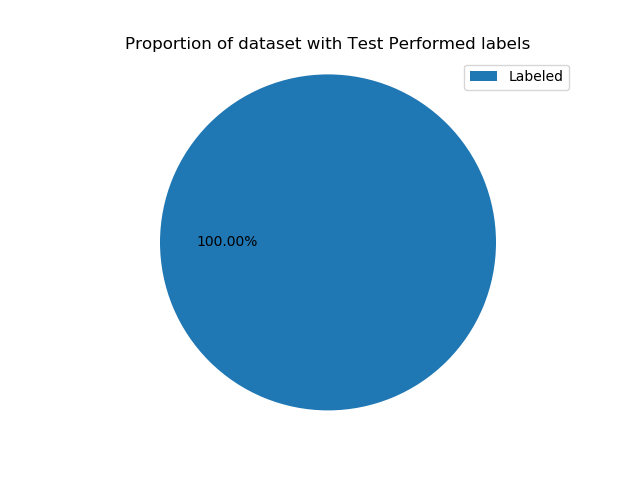
\includegraphics[width=8cm]{test_performed_labeled_prop.png} \\
    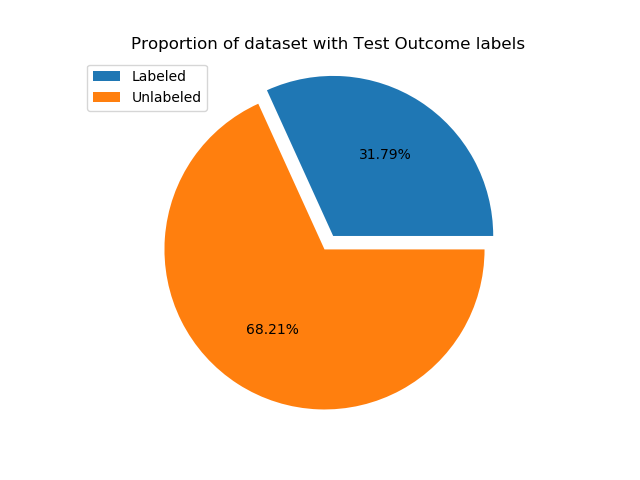
\includegraphics[width=8cm]{test_outcome_labeled_prop.png} \\
    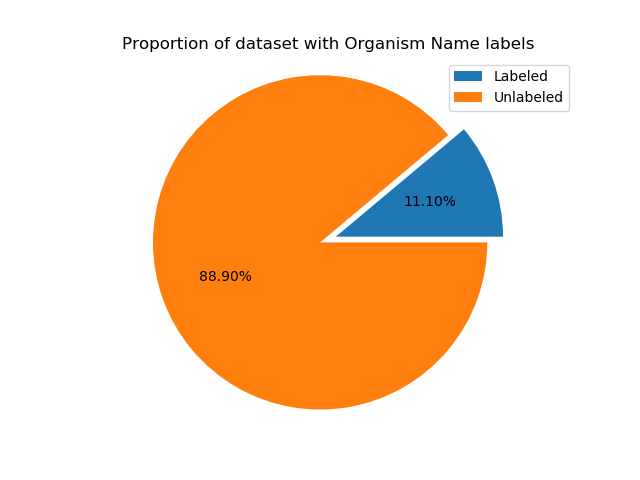
\includegraphics[width=8cm]{organism_name_labeled_prop.png} \\
    \caption{The proportion of labeled data for each output (approximately 950,000 rows total).}
    \label{proportion of labeled data figure}
\end{figure}


\subsection{Class Breakdown of Labeled Data} \label{class breakdown of labeled data}

\begin{figure}[H]
    \centering
    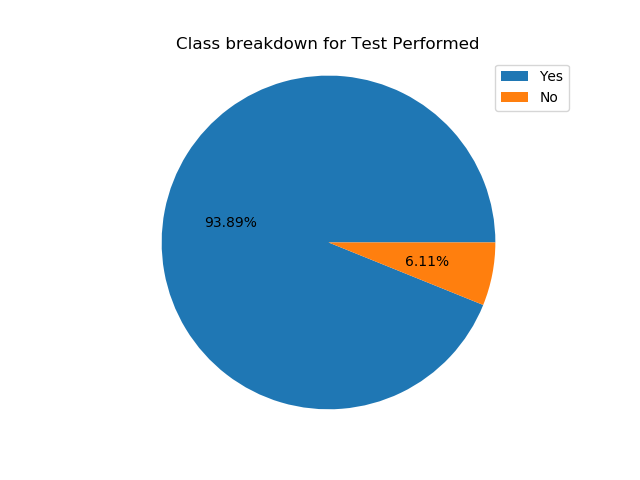
\includegraphics[width=8cm]{test_performed_classes_prop.png} \\
    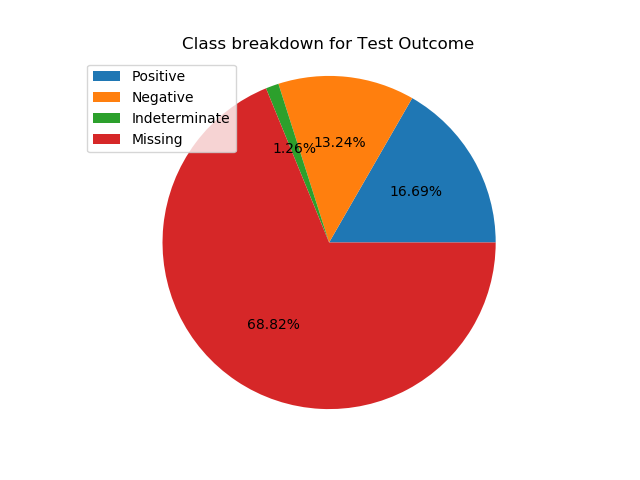
\includegraphics[width=8cm]{test_outcome_classes_prop.png} \\
    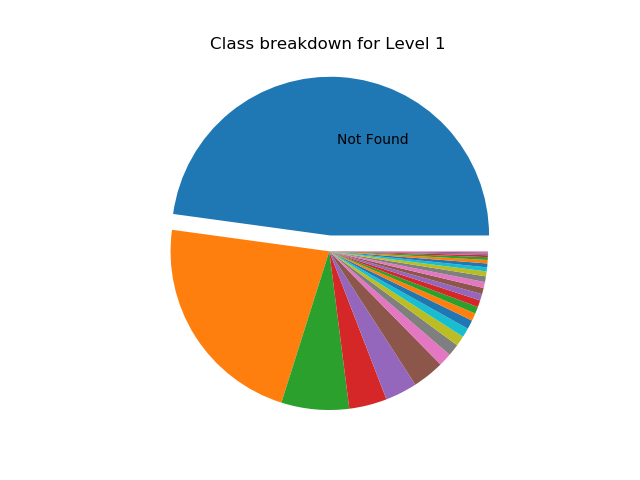
\includegraphics[width=8cm]{level_1_classes_prop.png} \\
    \caption{The class breakdown of labeled data for each output.}
    \label{class breakdown of labeled data figure}
\end{figure}


\newpage


\subsection{Test Outcome Binary Case Analysis} \label{test outcome binary case analysis}

\noindent \textit{Note: the analysis described in this section uses an early version of the data preprocessing step described in Section \ref{data preprocessing}. This section is included only to provide further insight into the data but the results may no longer be applicable.}
\\

Before we start our \verb|test_outcome| analysis with all four classes, we run preliminary experiments on the two-class case with classes \textit{Positive} and \textit{Negative}. The baseline classifier results are very similar to the four-class case as can been in Figure \ref{binary test outcome figure}.
\\

\begin{figure}[H]
    \centering
    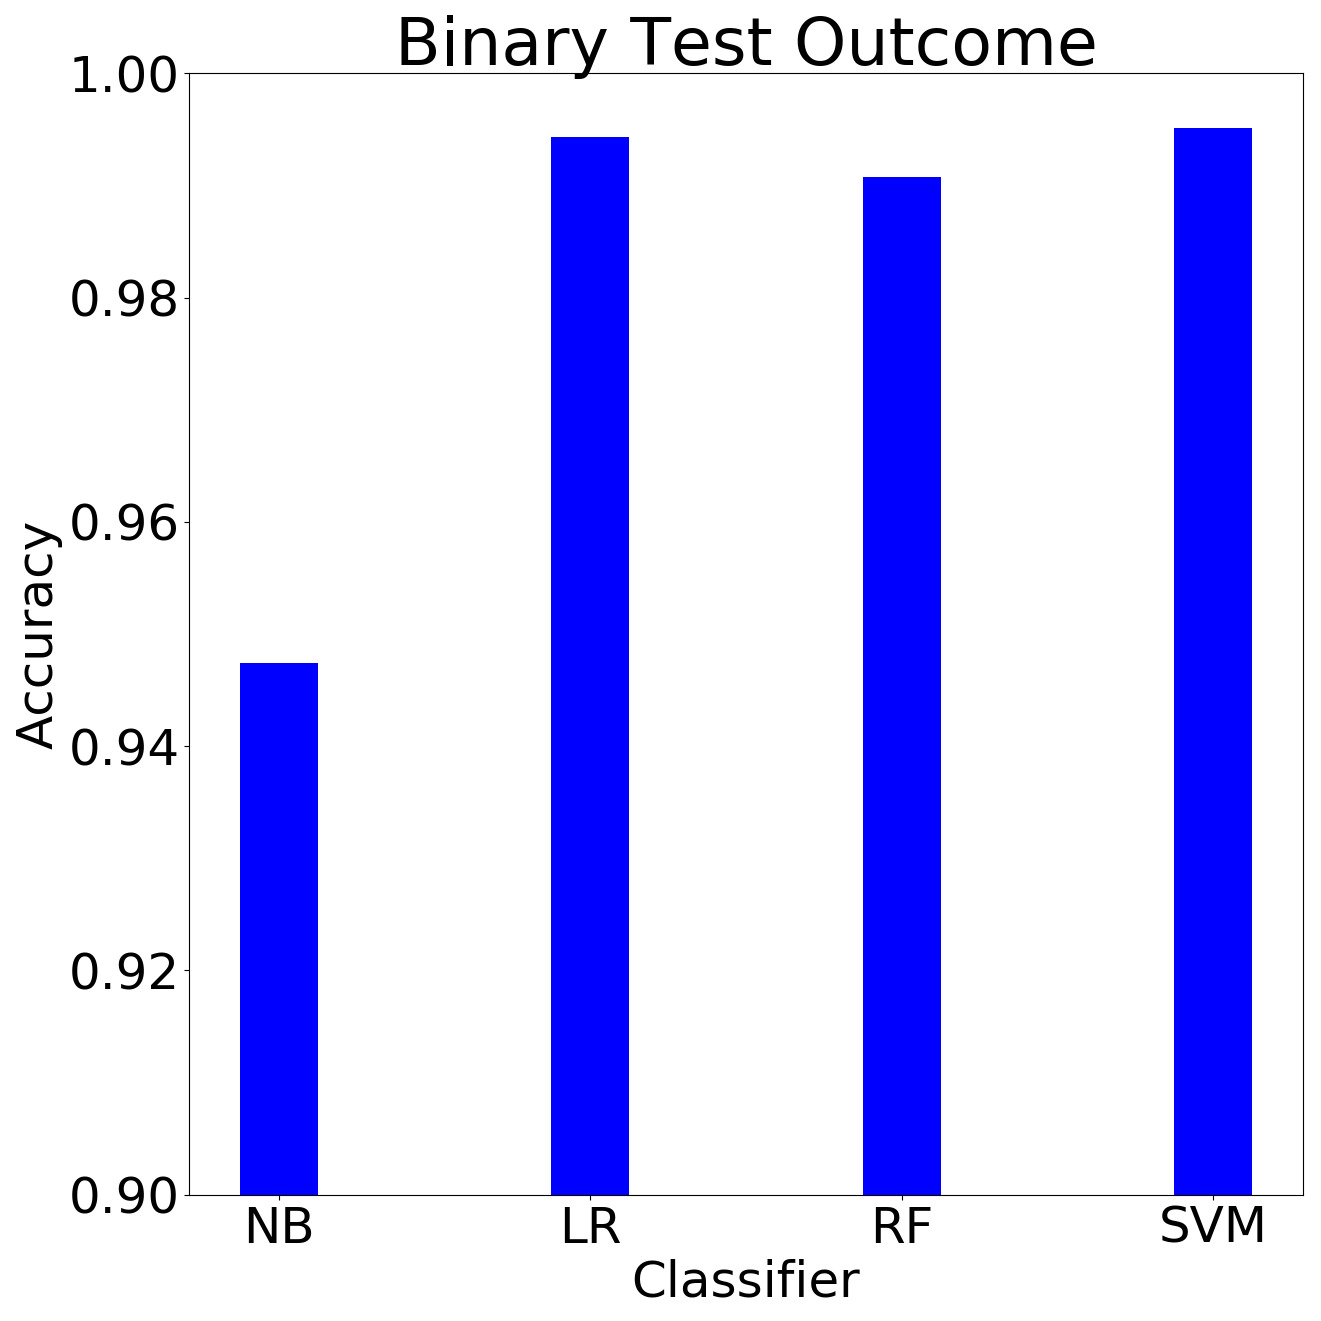
\includegraphics[width=8cm]{bto_graph.png}
    \SaveVerb{test outcome}|test_outcome|
    \caption{Baseline classifier performances for binary \protect\UseVerb{test outcome}.}
    \label{binary test outcome figure}
\end{figure}

Figure \ref{binary test outcome lr figure} shows the ``important" features as per LR weights. Note that this interpretation of feature importance should be taken cautiously as there may be strong correlations between features that may affect the LR weights in unexpected ways. We observe that although the most important features (``no", ``non", ``nonreactive", ``positive") are intuitively relevant for predicting \verb|test_outcome|, other features include some purely-numerical features (``16", ``30", ``2006", ``50") and some organism-specific features (``hbv" related to \textit{Hepatitis B}) which may be surprising. This implies that our classifiers are fitting to non-generalizable words. Future work may focus on using domain knowledge to produce a list of non-generalizable tokens to remove from the feature space.
\\

\begin{figure}[H]
    \centering
    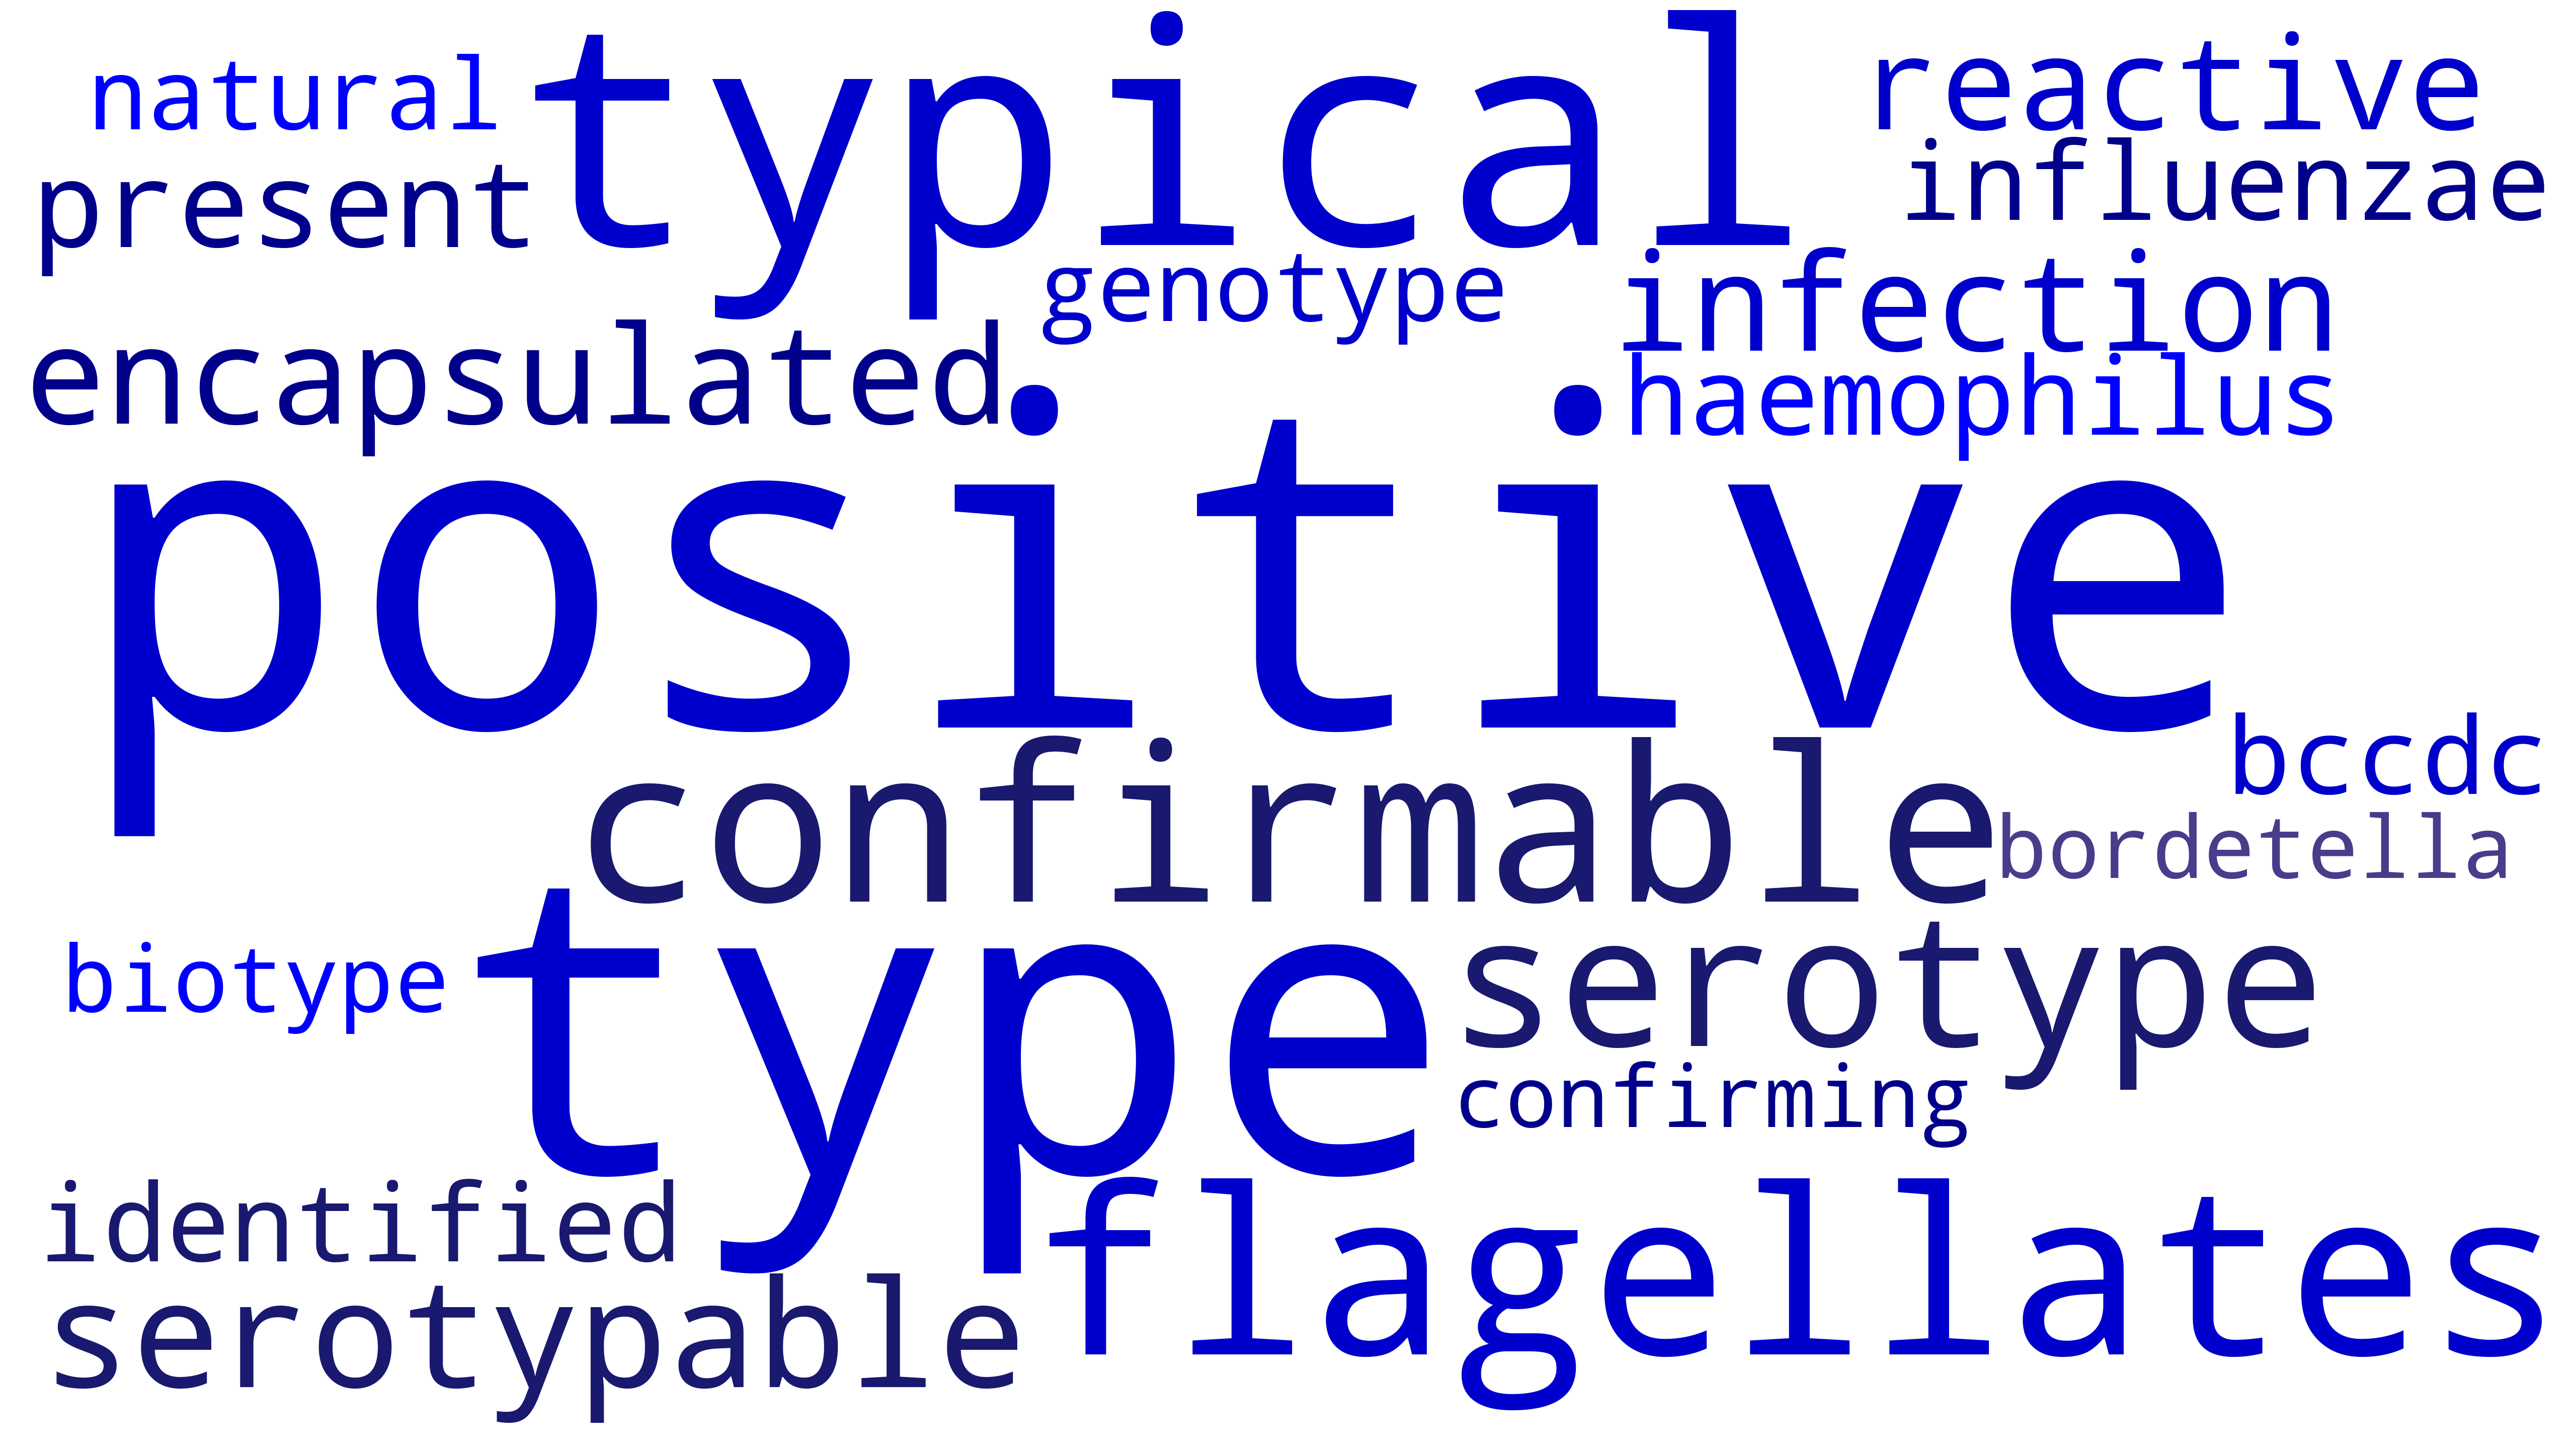
\includegraphics[width=0.49\textwidth]{logistic_regression_max.png}
    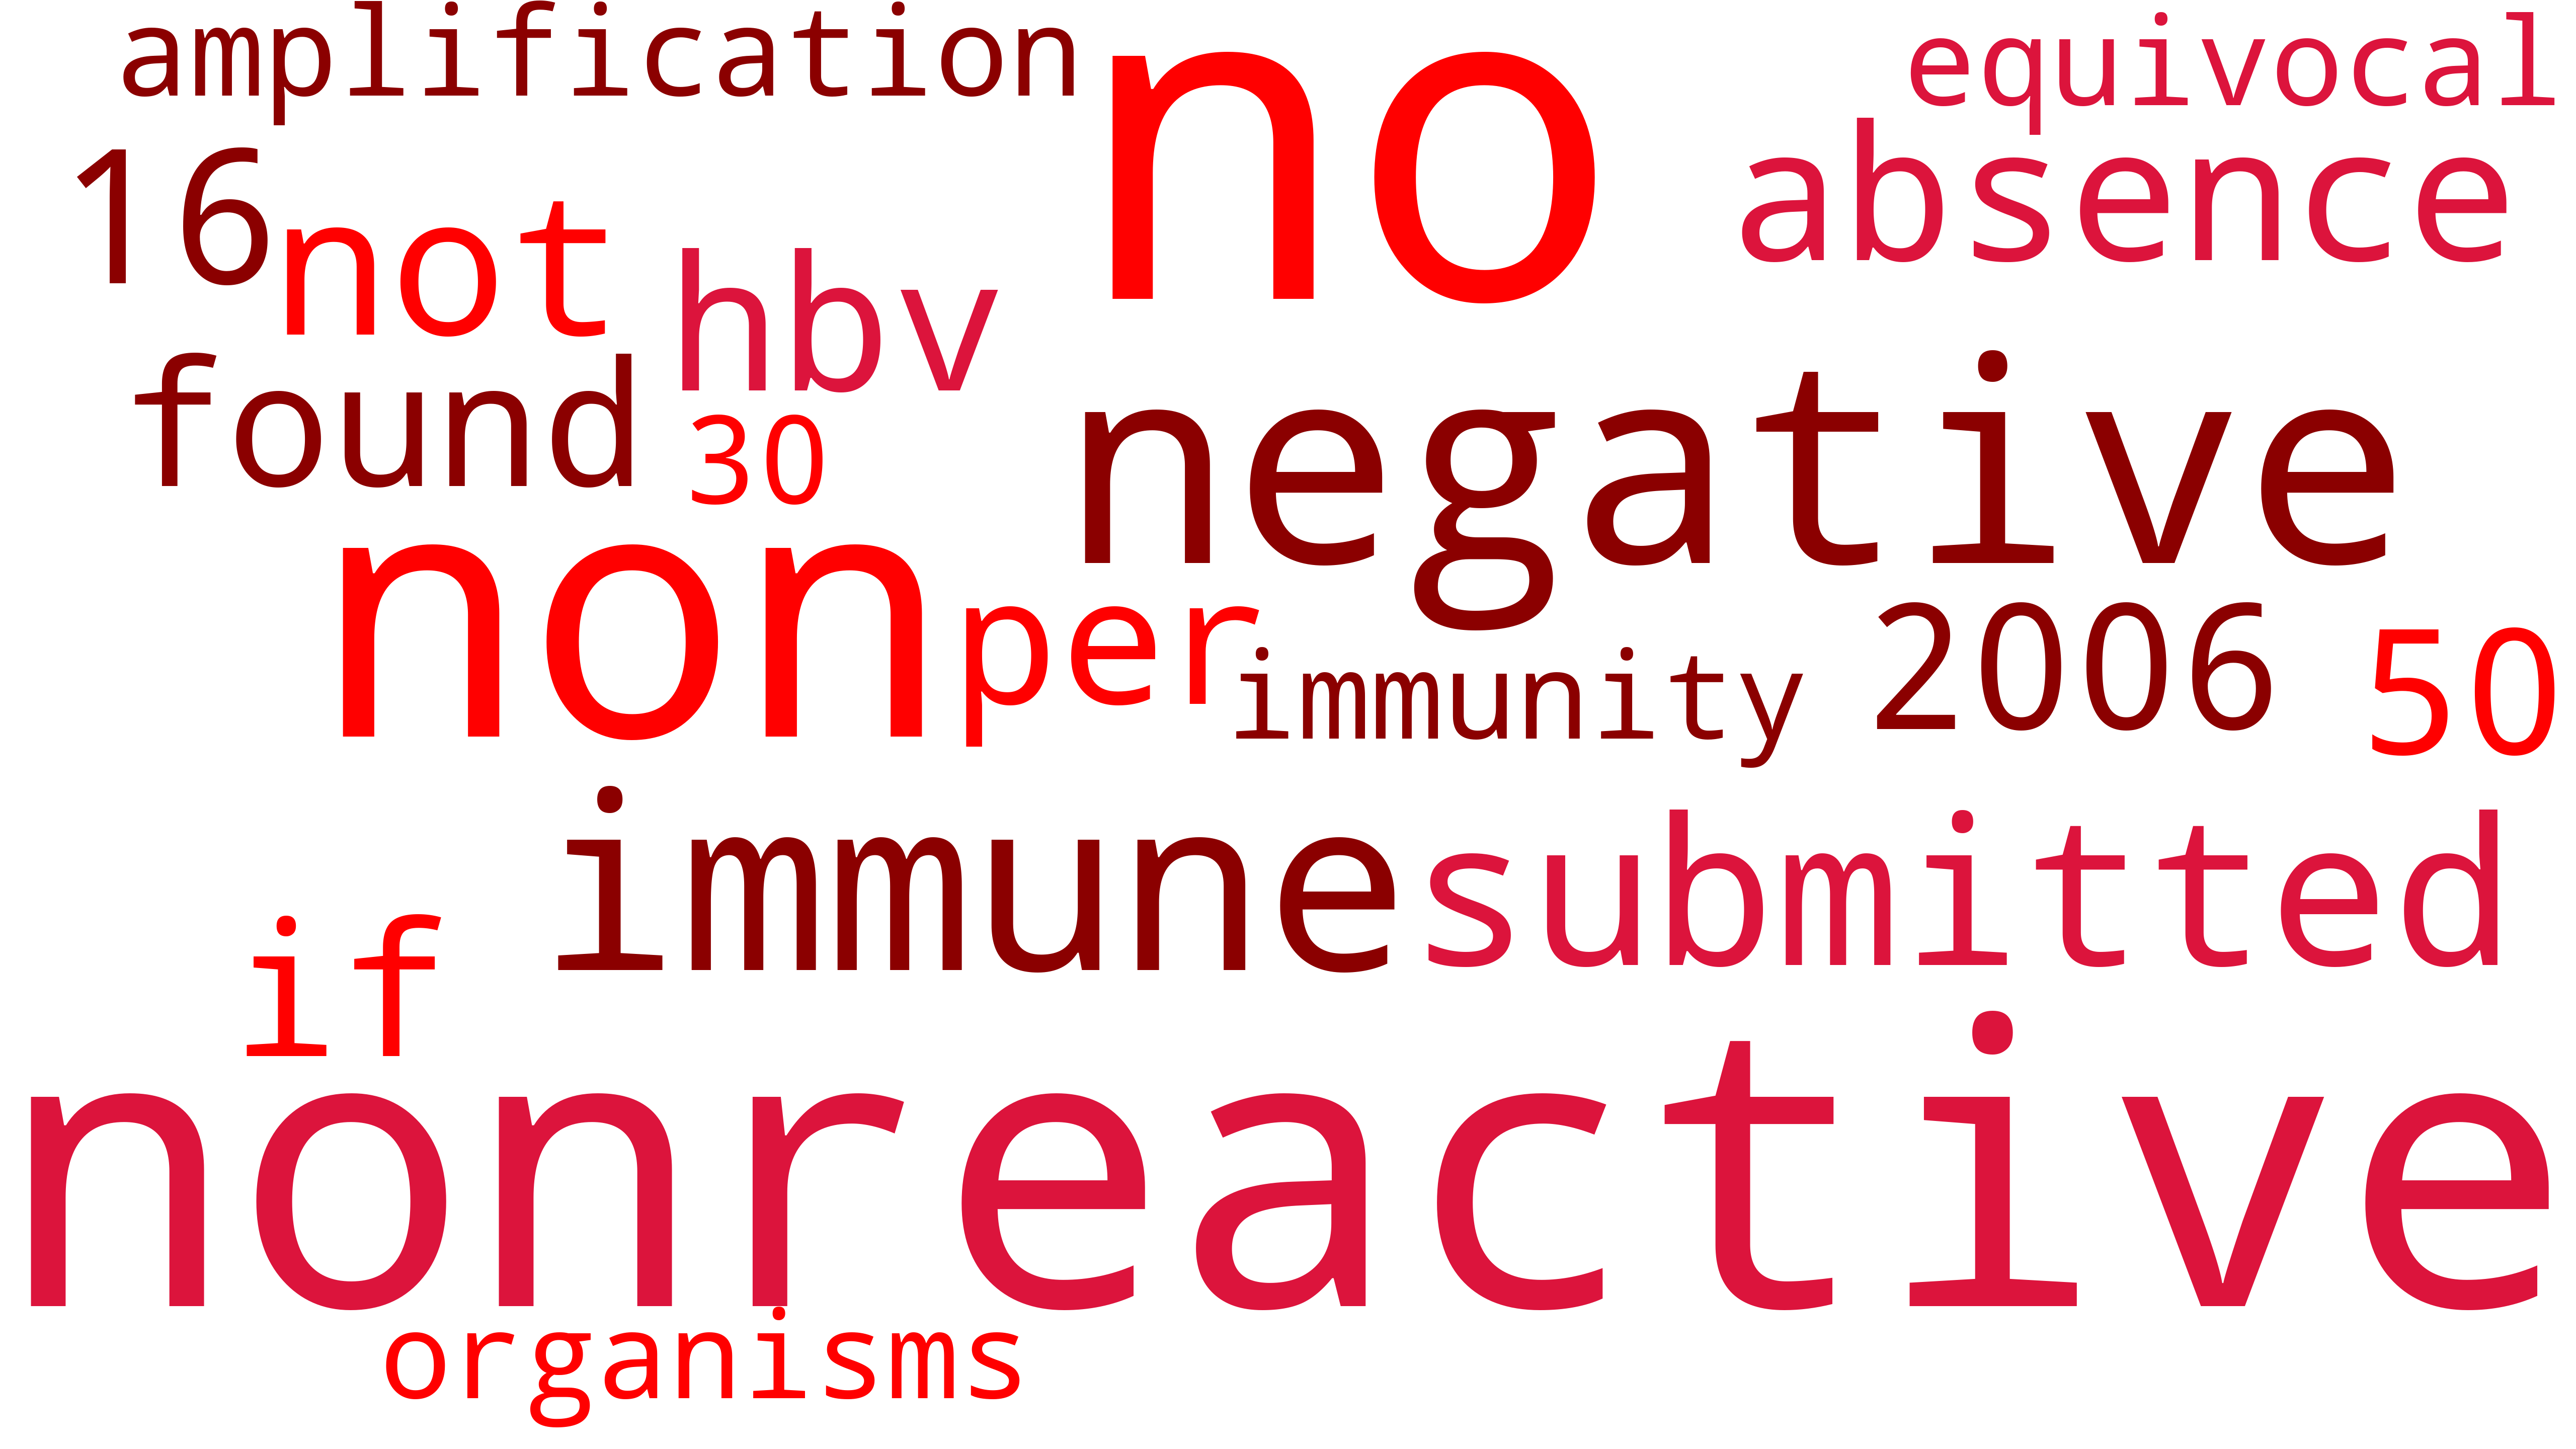
\includegraphics[width=0.49\textwidth]{logistic_regression_min.png}
    \SaveVerb{test outcome}|test_outcome|
    \caption{Most important features for \textit{Positive} (blue) and \textit{Negative} (red) \protect\UseVerb{test outcome} according to LR.}
    \label{binary test outcome lr figure}
\end{figure}


\newpage


\section{References} \label{references}

[1] Jang, H., Song, S. K. \& Myaeng, S. H. (2006). Text mining for medical documents using \\ \hspace*{10mm} a hidden
Markov model. \textit{Lecture Notes in Computer Science}, 4182, 553.
\\

[2] Kang, Y. S. \& Kayaalp, M. (2013). Extracting laboratory test information from biomedical \\ \hspace*{10mm} text. \textit{Journal of Pathology Informatics}, 4, 23.
\\

[3] Spasi\'c, I., Livsey, J., Keane, J. A. \& Nenadi\'c, G. (2014). Text mining of cancer-related \\ \hspace*{10mm} information: Review of current status and future directions. \textit{International Journal of Medical \\ \hspace*{10mm} Informatics}, 83(9), 605.


\end{document}

